\documentclass[11pt]{article}
\usepackage{setspace}
\setstretch{1}
\usepackage{amsmath,amssymb, amsthm}
\usepackage{graphicx}
\usepackage{bm}
\usepackage[hang, flushmargin]{footmisc}
\usepackage[colorlinks=true]{hyperref}
\usepackage[nameinlink]{cleveref}
\usepackage{footnotebackref}
\usepackage{url}
\usepackage{listings}
\usepackage[most]{tcolorbox}
\usepackage{inconsolata}
\usepackage[papersize={8.5in,11in}, margin=1in]{geometry}
\usepackage{float}
\usepackage{caption}
\usepackage{esint}
\usepackage{url}
\usepackage{enumitem}
\usepackage{subfig}
\usepackage{wasysym}
\newcommand{\ilc}{\texttt}
\usepackage{etoolbox}
\usepackage{algorithm}
\usepackage{changepage}
% \usepackage{algorithmic}
\usepackage[noend]{algpseudocode}
\usepackage{tikz}
\usetikzlibrary{matrix,positioning,arrows.meta,arrows}
\patchcmd{\thebibliography}{\section*{\refname}}{}{}{}
% \PassOptionsToPackage{hyphens}{url}\usepackage{hyperref}

\providecommand{\myceil}[1]{\left \lceil #1 \right \rceil }
\providecommand{\myfloor}[1]{\left \lfloor #1 \right \rfloor }


\begin{document}



\title{\textbf{CSDS 455: Homework 25}}


\author{Shaochen (Henry) ZHONG, \ilc{sxz517}}
\date{Due and submitted on 11/18/2020 \\ Fall 2020, Dr. Connamacher}
\maketitle



\section*{Problem 1}

\textit{Figure 9b is the $H(\alpha, 2q)$ graph for the shape of Figure 9a with $q=4$.  What is the $H(\alpha, 2q)$ graph when $q=5$?  Justify your answer.}\newline

\begin{figure}[H]
    \centering
    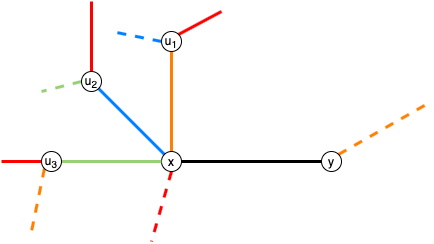
\includegraphics[width=0.4\linewidth]{{fig/fig_p1_1.png}}
\end{figure}

I believe this is the correct representation of $q = 5$ as we have 5 copies of $U$ and $V$. Since we only got 1 edge in Figure 9a so we don't have to worry about the edge with both endpoints on $U$ or $V$ (thus no double purple edges).


\section*{Problem 2}
\textit{Figres 12 and 13 are constraint graphs for the equivalent shape and H graph of Figure 9a and 9b with q=4.  What are equivalent constraint graphs when $q=5$}\newline

\noindent I don't quite get how injection works on this graph and how it is ``equal,'' but by mimicing the examples this seems to be true as we can have every edge appears twices.

\begin{figure}[H]
    \centering
    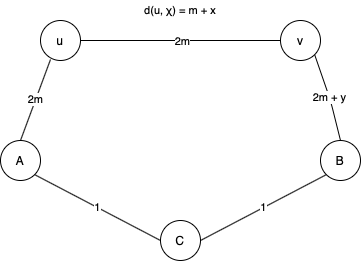
\includegraphics[width=0.4\linewidth]{{fig/fig_p2_1.png}}
\end{figure}

\end{document}